\section{Evaluation}
\label{sec:eval}

We have implemented our approach in \toolname: a system for repairing parse
errors for \python at its entirety. Next, we describe our implementation and an
evaluation that addresses four questions:

\begin{itemize}
    \item \textbf{RQ1}: How \emph{accurate} are \toolname's predicted error production rules?
                        (\S~\ref{sec:eval:accuracy})
    \item \textbf{RQ2}: How \emph{precisely} can \toolname repair parse errors?
                        (\S~\ref{sec:eval:precise})
    \item \textbf{RQ3}: How \emph{efficiently} can \toolname repair parse errors?
                        (\S~\ref{sec:eval:efficiency})
    \item \textbf{RQ4}: How \emph{useful} are \toolname's suggested repairs?
                        (\S~\ref{sec:eval:useful})
\end{itemize}

% \subsection{Implementation} \label{sec:eval:gen_method}

\mypara{Training Dataset}
For our evaluation, we use the \python dataset we used in our error data
analysis in \autoref{sec:error-analysis} gathered from
PythonTutor.com~\citep{Guo2013} between the years 2017 and 2018. The dataset has
more than 1,100,000 usable erroneous Python programs and their respective fixes.
The programs have an average length of \emph{87 tokens}, while the abstracted
token sequences have a much shorter average of \emph{43 tokens}. We use 15,000
random programs from the dataset for all our tests, and the rest we use as our
training set.

We first learn a PCFG on the training set of fixed programs in order to learn
the probabilities for each production rule in the \emph{full set of the \python
grammar}. \toolname then extracts the abstracted token sequences for all
programs in the training set. Next, while for the full set of \python there are
\emph{455 possible terminal error production rules} that \toolname's can predict
from, in reality only \emph{340 error rules} are ever used in the full dataset.
We arrive at this set of error rules by parsing all the erroneous programs in
the training set with the ECE-Parser and the "diff" error rules, as described in
\autoref{sec:overview:train}. Each program is also assigned as labels these
error rules that make the ECE-Parser parse the erroneous program successfully.

\mypara{Transformer Classifier}
\toolname's error rule prediction uses a Transformer classifier with \emph{six}
transformer blocks, that each has a fully-connected hidden layer of 256 neurons
and 12 attention heads. The output of the transformer blocks is then connected
to a \dnn based classifier with \emph{two} fully-connected hidden layers of 256
and 128 neurons respectively. The neurons use rectified linear units (ReLU) as
their activation function \citep{Nair2010-xg}, while the output layer uses the
sigmoid function for each class \citep{Nielsen2015-pu}. Additionally, the are
\emph{two input embedding layers} of a length of 128, one for input tokens and
one for their positions in the sequence. We also limit the size of the input
abstracted token sequences to a length of 128, which covers $95.7\%$ of the
training set, without the need of pruning them. Finally, the Transformer
classifier was trained using an \textsc{Adam} optimizer \citep{Kingma2014-ng}, a
variant of stochastic gradient descent that converges faster, for a total of 50
epochs.

\subsection{RQ1: Accuracy}
\label{sec:eval:accuracy}

We consider \toolname's transformer classifiers' accuracy up to the \emph{top
50} error production rules predictions against our original and the final
version of our approach

% colors from http://colorbrewer2.org/?type=sequential&scheme=Blues&n=3
\definecolor{blue1}{HTML}{DEEBF7}
\definecolor{blue2}{HTML}{9ECAE1}
\definecolor{blue3}{HTML}{3182BD}
\definecolor{green1}{HTML}{E5F5E0}
\definecolor{green2}{HTML}{A1D99B}
\definecolor{green3}{HTML}{31A354}

\begin{figure}[t]
  % \begin{minipage}[c]{0.49\linewidth}
    \centering
    \resizebox{0.6\linewidth}{!}{
      \Large
      \begin{tikzpicture}
      \begin{axis}[
        ybar stacked,
        width=1.1\linewidth,
        height=11cm,
        % title={Accuracy of Repair Template Prediction},
        ylabel={Prediction Accuracy (\%)},
        bar width=1cm,
        ymin=0.0,
        ymax=101.0,
        ytick={0.0, 10.0, 20.0, 30.0, 40.0, 50.0, 60.0, 70.0, 80.0, 90.0, 100.0},
        yticklabel={\pgfmathparse{\tick}\pgfmathprintnumber{\pgfmathresult}},
        ytick style={draw=none},
        ymajorgrids = true,
        symbolic x coords={original, abstracted, abstracted-best},
        enlarge x limits=0.3,
        xtick=data,
        xtick style={draw=none},
        xticklabels={\textsc{Original}\xspace, \textsc{Abstracted}\xspace, \textsc{Threshold}\xspace},
        %x tick label style={rotate=45, anchor=north east},
        % x tick label style={font=\small},
        % y tick label style={font=\small},
        reverse legend,
        % transpose legend,
        legend style={legend pos = north east, legend columns=4, font=\small},
      ]

      \addplot[draw=black, fill=blue2, bar shift=-.501cm, postaction= { pattern=dots }] coordinates {(original, 0.0) (abstracted, 0.0) (abstracted-best, 79.28025102961365)};

      \resetstackedplots

      \addplot[draw=black, fill=green2, bar shift=.501cm, postaction= { pattern=dots }] coordinates {(original, 0.0) (abstracted, 0.0) (abstracted-best, 69.82968369829683)};

      \resetstackedplots

      \addplot[draw=black, fill=green1, bar shift=.501cm] coordinates {(original, 12.875536480686696) (abstracted, 58.394160583941606) (abstracted-best, 0.0)};
      \addlegendentry{Top-10}
      \addplot[draw=black, fill=green2, bar shift=.501cm] coordinates {(original, 20.100143061516448) (abstracted, 14.922952149229523) (abstracted-best, 0.0)};
      \addlegendentry{Top-20}
      \addplot[draw=black, fill=green3, bar shift=.501cm] coordinates {(original, 31.974248927038623) (abstracted, 15.49067315490673) (abstracted-best, 0.0)};
      \addlegendentry{Top-50}
      \addlegendimage{empty legend}
      \addlegendentry{Rare:}

      \resetstackedplots

      \addplot[draw=black, fill=blue1, bar shift=-.501cm] coordinates {(original, 56.712132089016514) (abstracted, 72.11217885859972) (abstracted-best, 0.0)};
      \addlegendentry{Top-10}
      \addplot[draw=black, fill=blue2, bar shift=-.501cm] coordinates {(original, 11.769733018835673) (abstracted, 9.335163757599531) (abstracted-best, 0.0)};
      \addlegendentry{Top-20}
      \addplot[draw=black, fill=blue3, bar shift=-.501cm] coordinates {(original, 18.65107852186101) (abstracted, 11.253840622344256) (abstracted-best, 0.0)};
      \addlegendentry{Top-50}
      \addlegendimage{empty legend}
      \addlegendentry{All:}

      \end{axis}
      \end{tikzpicture}
    }
    \caption{
      Results of our error production rule prediction classifiers for the simple original token sequences and their abstracted versions using the PCFG.
    }
    \label{fig:accuracy-results}
  % \end{minipage}
  % \begin{minipage}[c]{0.49\linewidth}
  %   \centering
  %   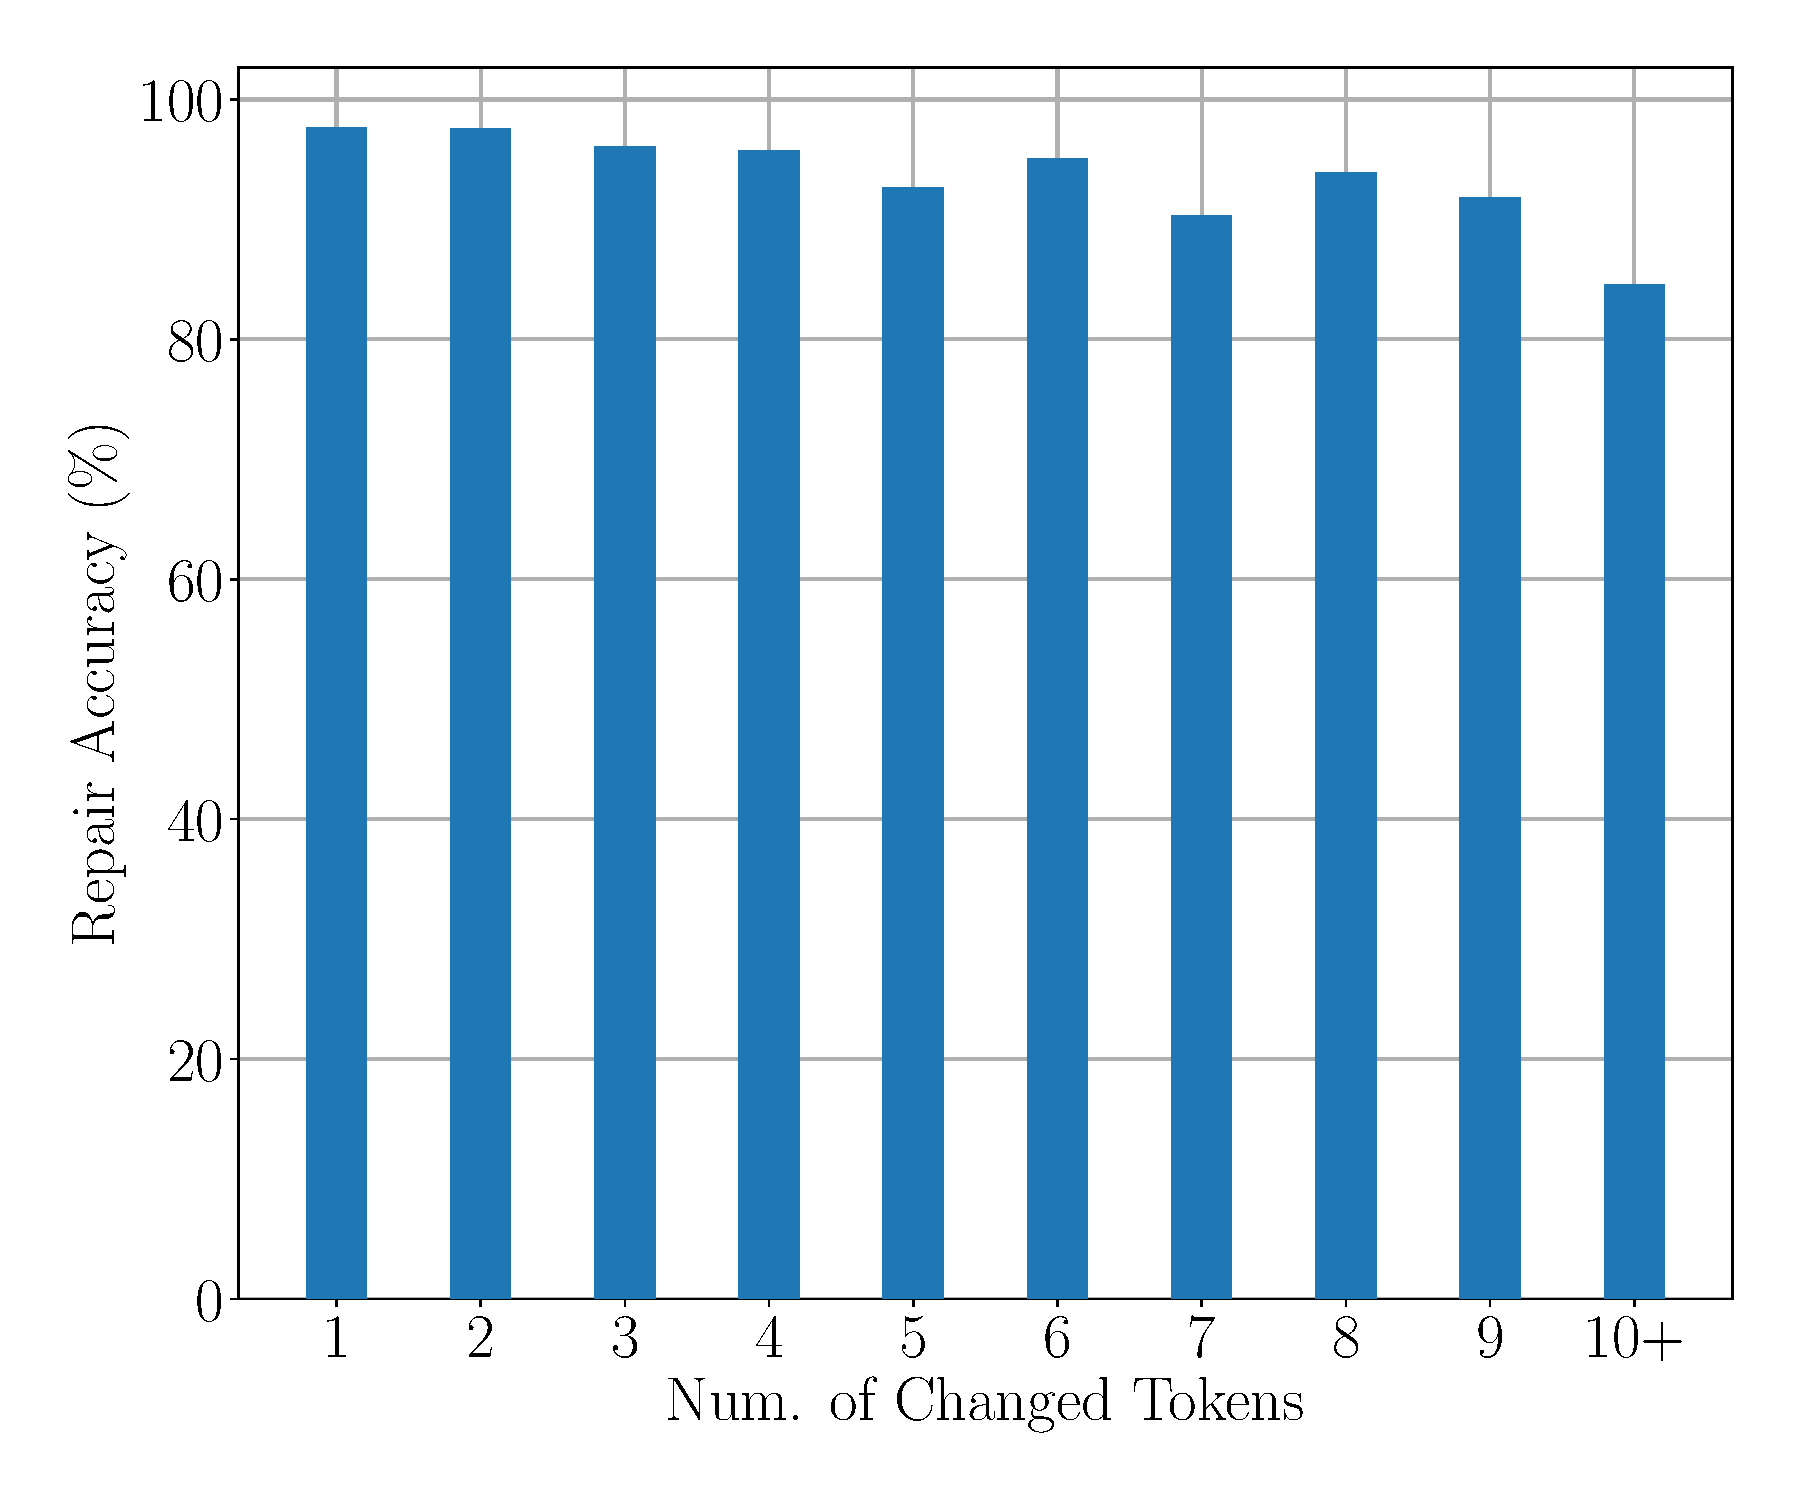
\includegraphics[width=\linewidth]{accuracy-per-change.pdf}
  %   \caption{The repair accuracy for the number of edits needed by the user to repair.}
  %   \label{fig:accuracies-per-changes}
  % \end{minipage}
\end{figure}


\mypara{Results: Accuracy of Error Rule Prediction}
%
\autoref{fig:accuracy-results} shows the accuracy results of our error
production rule prediction experiments. The y-axis describes the fraction of
programs for which the \emph{whole} set of the needed error rules needed to
repair the \emph{erroneous} program was a complete subset of the top-K predicted
rules.
%
The \textsc{Original} version of our transformer classifier didn't consider the
partial parses produced with the PCFG's aid and used the full \textsc{Original}
token sequences, whose results are presented in the first two bars of
\autoref{fig:accuracy-results}. The next two bars show our final results using
the \textsc{Abstracted} token sequences to train the classifier. Finally, the
last two dotted bars show the results for when a \textsc{Threshold} is set in
order to select the predicted error rules, instead of picking the static top-K
ones. The predicted error rule set can have a size anywhere between 1 and a
maximum of 25 (pre-defined by us based on the top-K results).

The blue bars show the accuracy on the full test set of \textsc{All} 15,000
programs, while the green bars show the results on the subset of \textsc{Rare}
programs, \ie the programs that didn't include any of the 50 most popular error
rules, that amount only for 4.8\% of our test set.

The \textsc{Original} predictor, even with the Top-50 predicted error rules is
less accurate than the Top-20 predictions of the \textsc{Abstracted}, with an
accuracy of 73.96\%, which drops to 51.16\% and 32.34\% respectively for the
Top-20 and Top-10 predictions. The \textsc{Abstracted} predictor significantly
outperforms the \textsc{Original} predictor with a 72.08\% Top-10 accuracy,
81.08\% Top-20 accuracy and 92.13\% Top-10 accuracy.

The \textsc{Threshold} predictions are almost as accurate as the
\textsc{Abstracted} Top-20 predictions with an accuracy of 79.46\% and a median
number of selected error rules of 12 (average 13.9). This could potentially mean
that this predictor is a valid alternative for the static Top-20 predictions.

Finally, we observe that our \textsc{Abstracted} classifiers generalize
efficiently for our dataset of erroneous \python programs and is almost as
accurate as the rest of the dataset with a 74.11\% Top-20 accuracy (85.69\%
Top-50 accuracy). The same holds for the \textsc{Threshold} predictions with a
72.46\% accuracy.

\begin{framed}
  \noindent \toolname's transformer classifier learns to encode programs with
  syntax errors and select candidate error production rules for them
  effectively, yielding \emph{high accuracies}. By abstracting the tokens
  sequences, \toolname is able to \emph{generalize} better and make more
  accurate predictions with a \emph{81.08\% Top-20 accuracy}.
\end{framed}


\subsection{RQ2: Repaired Program Preciseness}
\label{sec:eval:precise}

\begin{table}[t]
  \centering
  \begin{tabular}{l||cccc}
    Error Rule Approach            & Parse Accuracy & User Parse Rate & Parse time & Speedup \\
    \hline
    20 Most Popular                & 79.81\% & 16.31\% & 4.8 sec  & 45.8 sec \\
    50 Most Popular                & 90.03\% & 18.55\% & 10.6 sec & 37.1 sec \\
    Top-20 (\textsc{All-Parses})   & 59.31\% & 30.57\% & 15.6 sec & 57.4 sec \\
    Top-20 (\textsc{Minimum-Cost}) & 92.45\% & 19.95\% & 4.1 sec  & 68.0 sec \\
  \end{tabular}
  \caption{Experimental results of \toolname's repair approaches.}
  \label{tab:seq2parse_full_results}
\end{table}

Next we evaluate \toolname's end-to-end accuracy and preciseness in generating
valid parses for programs with syntax errors. For all of our tests we limit the
\toolname's parsing to \emph{5 mins} and run our experiments on \emph{15,000
erroneous programs} from our dataset. The rest of the dataset was used to train
our transformer classifiers, and specifically here the \textsc{Abstracted}
classifier.

We compare our \emph{two versions} of our implementation of \toolname
(\textsc{All-Parses} and \textsc{Minimum-Cost}) against two versions of the
error-correcting parser with a static selection of the 20 and 50 most popular
error production rules in our training set. We make this comparison because we
observe in our training set that the 50 most of popular error rules are used for
parsing as much as \emph{86\%} of the dataset.

Our \textsc{All-Parses} ECEP and \textsc{Minimum-Cost} ECEP both use the
\emph{Top-20 predictions} from our \textsc{Abstracted} classifier to generate
parses and thus generate full program repairs. The \textsc{All-Parses} ECEP
keeps internally all possible states that arise from using the predicted error
rules and having a maximum repair cost of 2 edits (\ie a maximum of 2
insertions, deletions or replacements). The \textsc{Minimum-Cost} version
however keeps always the minimum-edit repair and discards all other states that
may lead to a higher cost. This allows for a higher maximum cost of 10 edits.
Finally, while \textsc{All-Parses} can generate a large number of repairs, we
keep only the top 3 repairs after filtering with a static code checker
(\textsc{Pylint}, \url{https://www.pylint.org/}) as most developers will
consider at most five suggestions before falling back to manual debugging
\citep{Kochhar2016-oc, Parnin2011-ce}.

\autoref{tab:seq2parse_full_results} shows the percentage of test programs that
each of these four versions can parse successfully (\ie the parse accuracy) and
the amount of parses that match the one that user compiled. We observe that the
Top-20 predictions with the \textsc{Minimum-Cost} ECEP \emph{outperforms} every
other option in parse accuracy and parse time, with 92.45\% and 4.1 seconds
respectively. It also achieves to generate the intended parse for 19.95\% of the
set, \ie in almost 1 out 5 of the cases. The 20 most popular ECEP with 79.81\%
parse accuracy and 4.8 seconds parse time is less accurate while a bit slower in
general, and achieves 3.64\% less times to generate the user parse, while the 50
most popular is slightly less accurate with 90.03\%, but a lot slower in general
with 10.6 seconds parse time. The 50 most popular ECEP also almost achieves the
\textsc{Minimum-Cost} ECEPs with a 18.55\% user parse rate. The
\textsc{All-Parses} ECEP has a smaller parse accuracy of 59.31\%, however it
manages to generate the user fix 30.57\% of the times, \ie almost one out of
three programs with syntax errors, with the cost that is also the slowest
version with a parse time of 15.6 seconds.

\begin{framed}
  \noindent \toolname can \emph{generate parses} for \emph{92\%} of our tests
  within 4.1 secs for the majority of them, while also generating \emph{the user
  fix in almost 1 out 5 of the cases}.
\end{framed}

\subsection{RQ3: Efficiency}
\label{sec:eval:efficiency}

\begin{figure}[t]
  \centering
  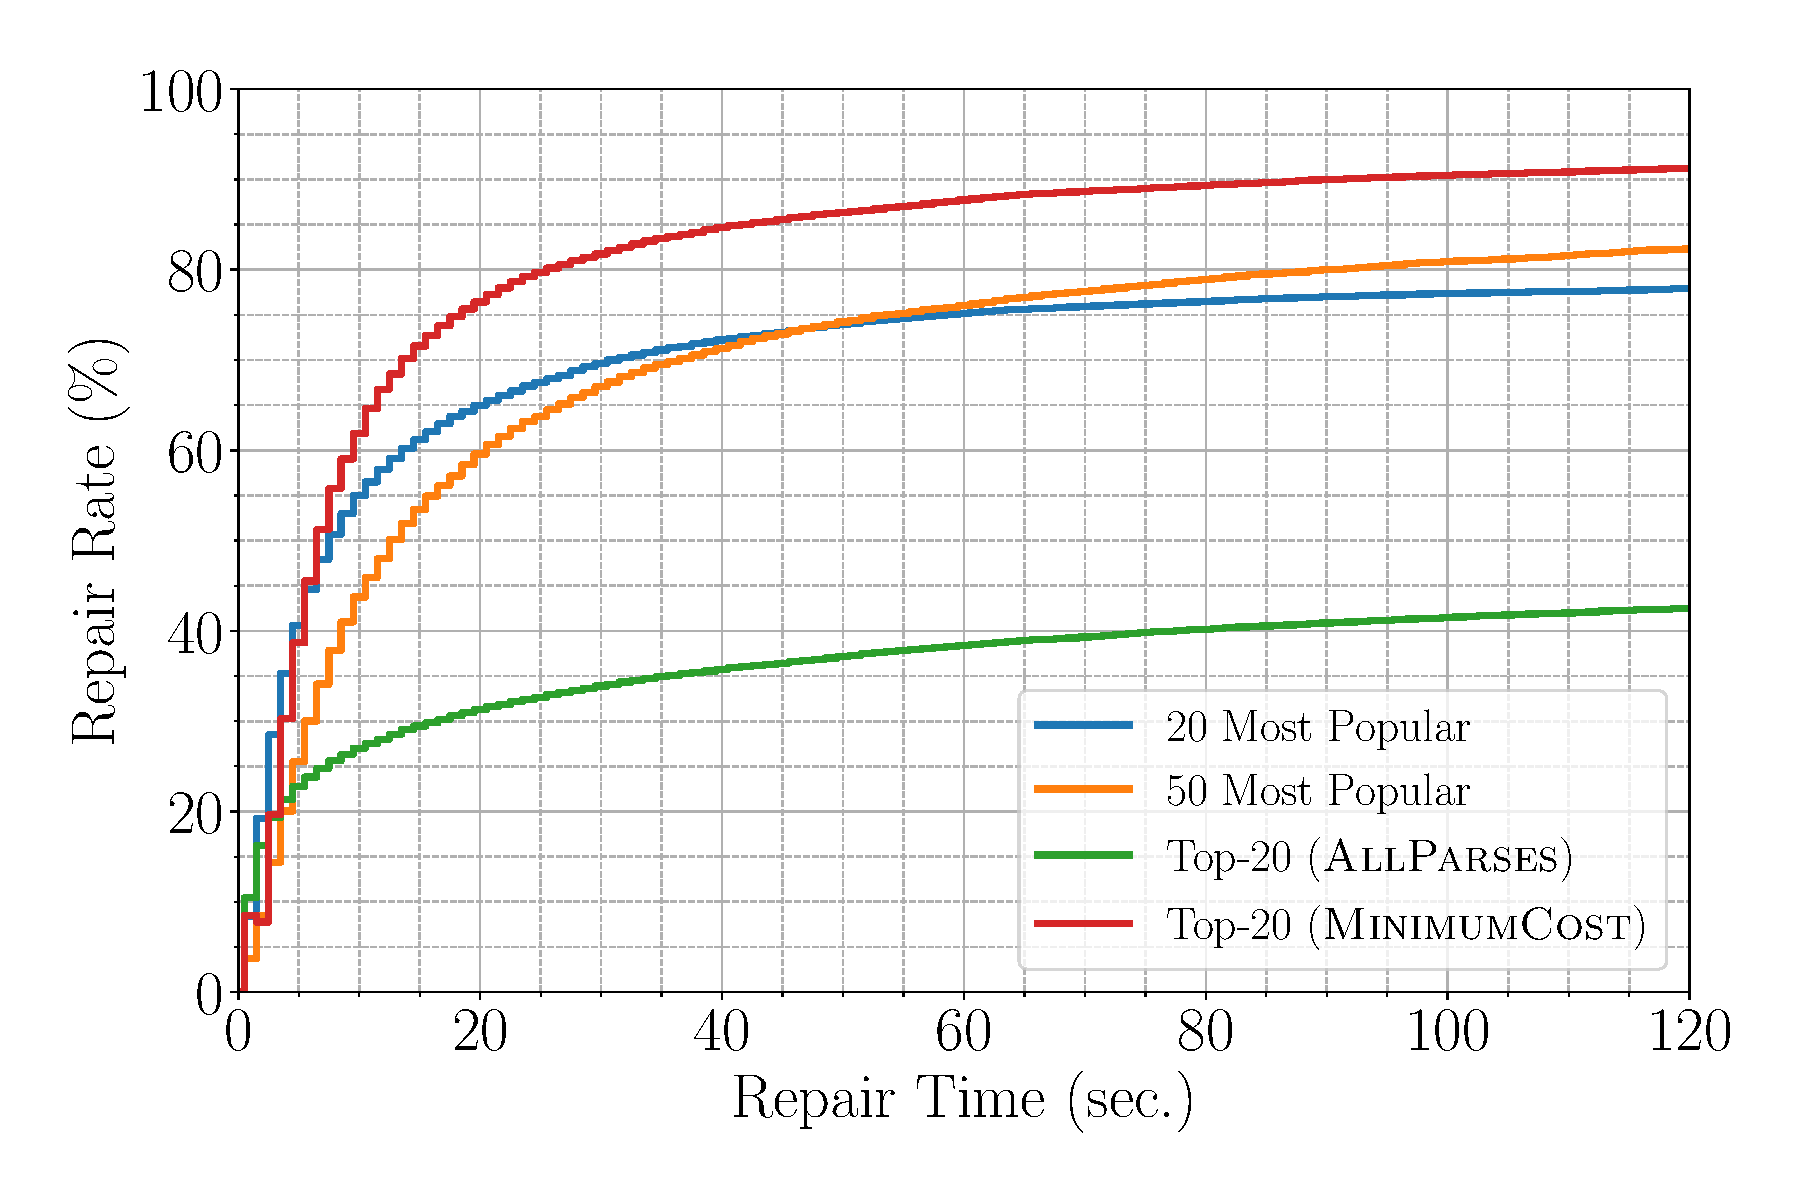
\includegraphics[width=0.8\linewidth]{tool-repair-rate.pdf}
  \caption{The repair rate for all the approaches in
  \autoref{tab:seq2parse_full_results}}
  \label{fig:tool-repair-rate}
\end{figure}

Next we evaluate \toolname's efficiency by measuring how many programs it is
able to parse. We limit each ECEP to 180 seconds. (In general the procedure is
undecidable, and we conjecture that a longer timeout will diminish the practical
usability for novices.) We compare the efficiency of \toolname for all the
versions of \autoref{tab:seq2parse_full_results}.

\autoref{fig:tool-repair-rate} shows the cumulative distribution function of all
\toolname approaches' repair rates over their parse time. We observe that using
the top 20 error production rule predictions is the most efficient while
maintaining the highest parse accuracy at all times, with a repair rate of
80.8\% within 25 seconds.

We observe that, using a fixed set of the 20 and 50 most popular rules for
\toolname to parse programs with syntax errors, a 67.9\% and 64.5\% respectively
within 25 seconds. The 50 most popular ECEP is parses less programs until the 45
seconds but the extra number of error rules aids the ECEP to parse more after
that point and outperform the 20 most popular ECEP.

We also observe that \toolname successfully parses around 33.0\% of the programs
with its \textsc{All-Parses} approach in 25 seconds. While this approach is much
less efficient that the others. due to the vast amount of states is keeps
internally in its data structure, it is also able to generate the exact human
repair in 1 out of 3 times which makes still a very valuable approach
(\S~\ref{sec:eval:precise}).

\begin{framed}
  \noindent \toolname can parse programs with syntax errors for the vast
  majority of the test set in under 25 seconds.
\end{framed}

\subsection{RQ4: Usefulness}
\label{sec:eval:useful}
